\hypertarget{st__flush_8c}{
\section{st\_\-flush.c File Reference}
\label{st__flush_8c}\index{st_flush.c@{st\_\-flush.c}}
}


\subsection{Detailed Description}
\begin{Desc}
\item[For internal use only.]
This file contains the implementation of the \hyperlink{group__dbprim__smat_ga15}{st\_\-flush()} function, used to release all entries in a sparse matrix table.\end{Desc}


Definition in file \hyperlink{st__flush_8c-source}{st\_\-flush.c}.

{\tt \#include \char`\"{}dbprim.h\char`\"{}}\par
{\tt \#include \char`\"{}dbprim\_\-int.h\char`\"{}}\par


Include dependency graph for st\_\-flush.c:\begin{figure}[H]
\begin{center}
\leavevmode
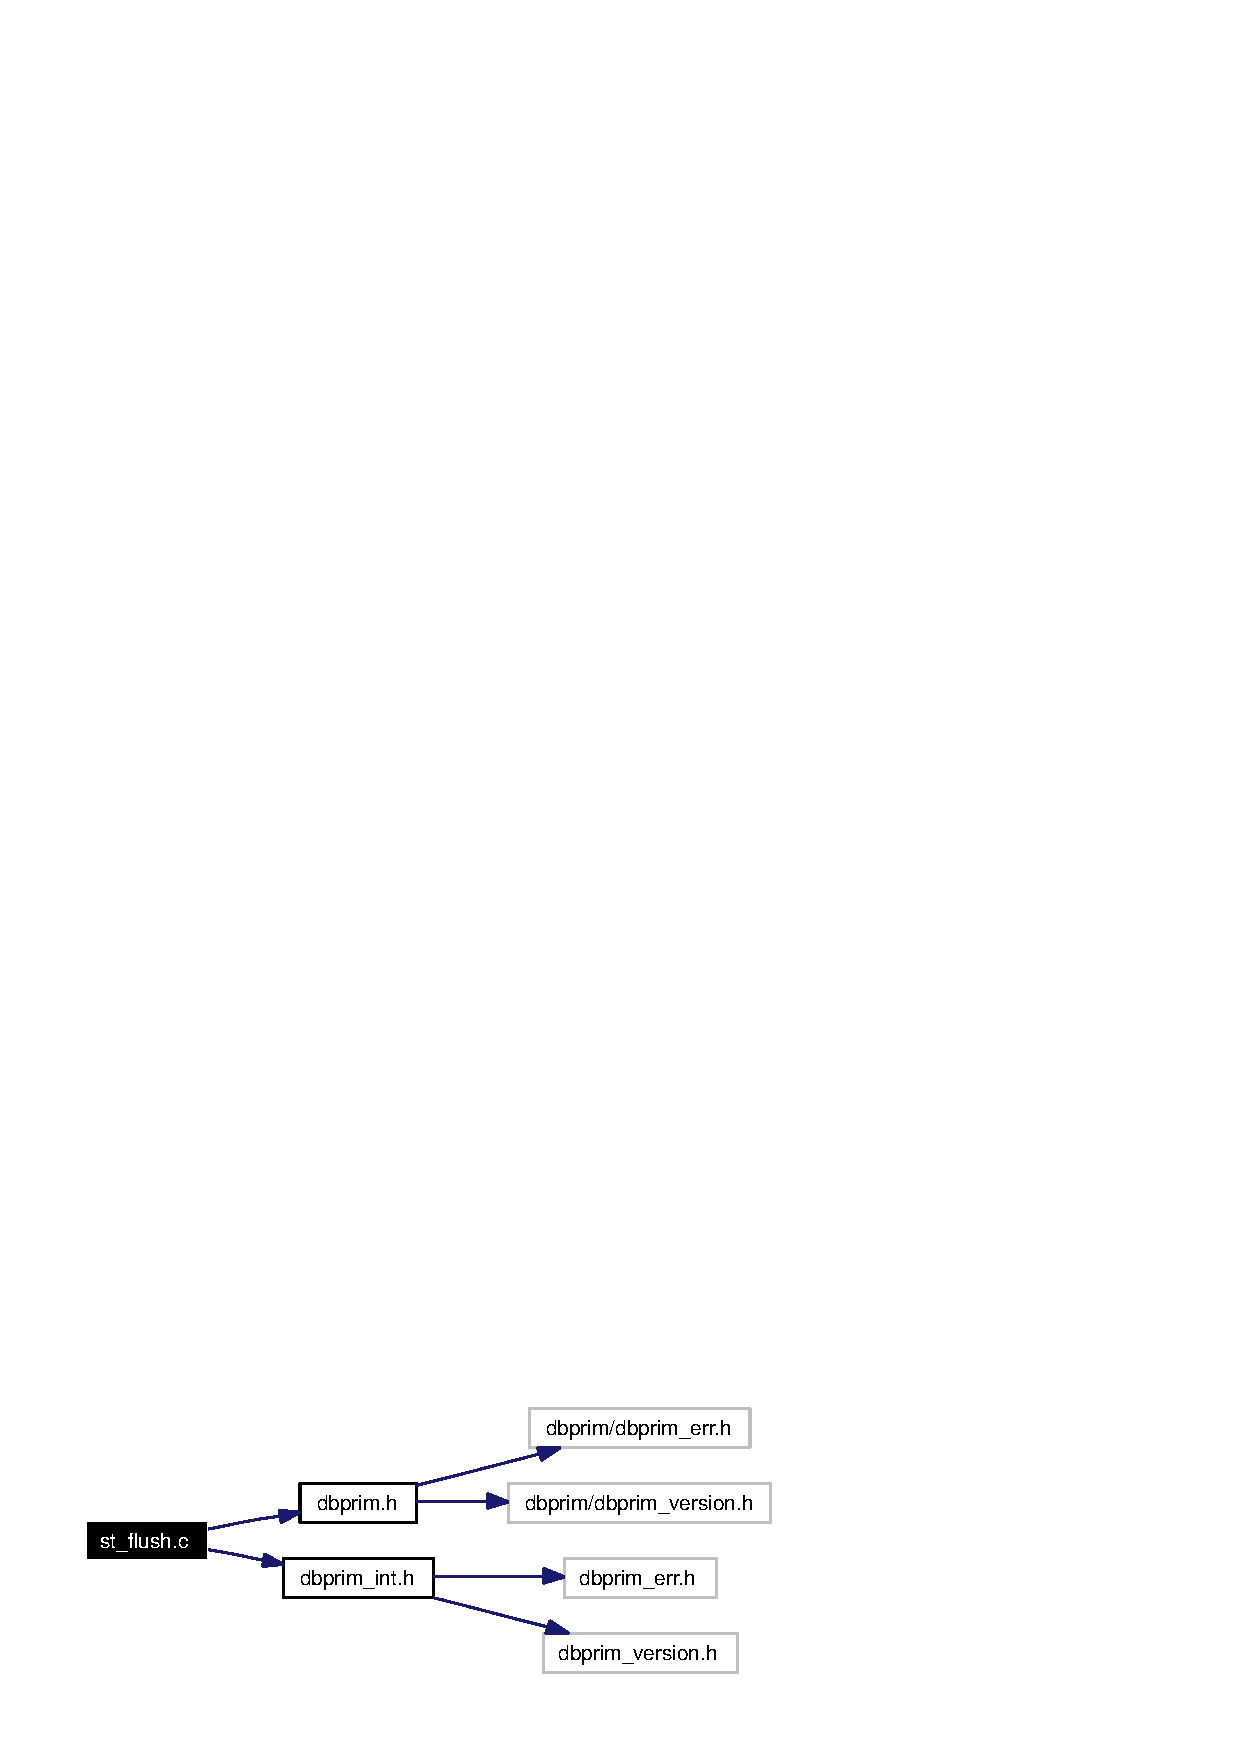
\includegraphics[width=187pt]{st__flush_8c__incl}
\end{center}
\end{figure}
\subsection*{Data Structures}
\begin{CompactItemize}
\item 
struct \hyperlink{struct__st__flush__s}{\_\-st\_\-flush\_\-s}
\begin{CompactList}\small\item\em Sparse matrix flush function shim structure. \item\end{CompactList}\end{CompactItemize}
\subsection*{Functions}
\begin{CompactItemize}
\item 
static unsigned long \hyperlink{group__dbprim__smat_ga30}{\_\-st\_\-flush\_\-iter} (\hyperlink{struct__hash__table__s}{hash\_\-table\_\-t} $\ast$table, \hyperlink{struct__hash__entry__s}{hash\_\-entry\_\-t} $\ast$ent, void $\ast$extra)
\begin{CompactList}\small\item\em Sparse matrix hash flush callback. \item\end{CompactList}\item 
unsigned long \hyperlink{group__dbprim__smat_ga15}{st\_\-flush} (\hyperlink{struct__smat__table__s}{smat\_\-table\_\-t} $\ast$table, \hyperlink{group__dbprim__smat_ga4}{smat\_\-iter\_\-t} flush\_\-func, void $\ast$extra)
\begin{CompactList}\small\item\em Flush a sparse matrix. \item\end{CompactList}\end{CompactItemize}
